\section{Overview}
\begin{figure}[H]
    \centering
    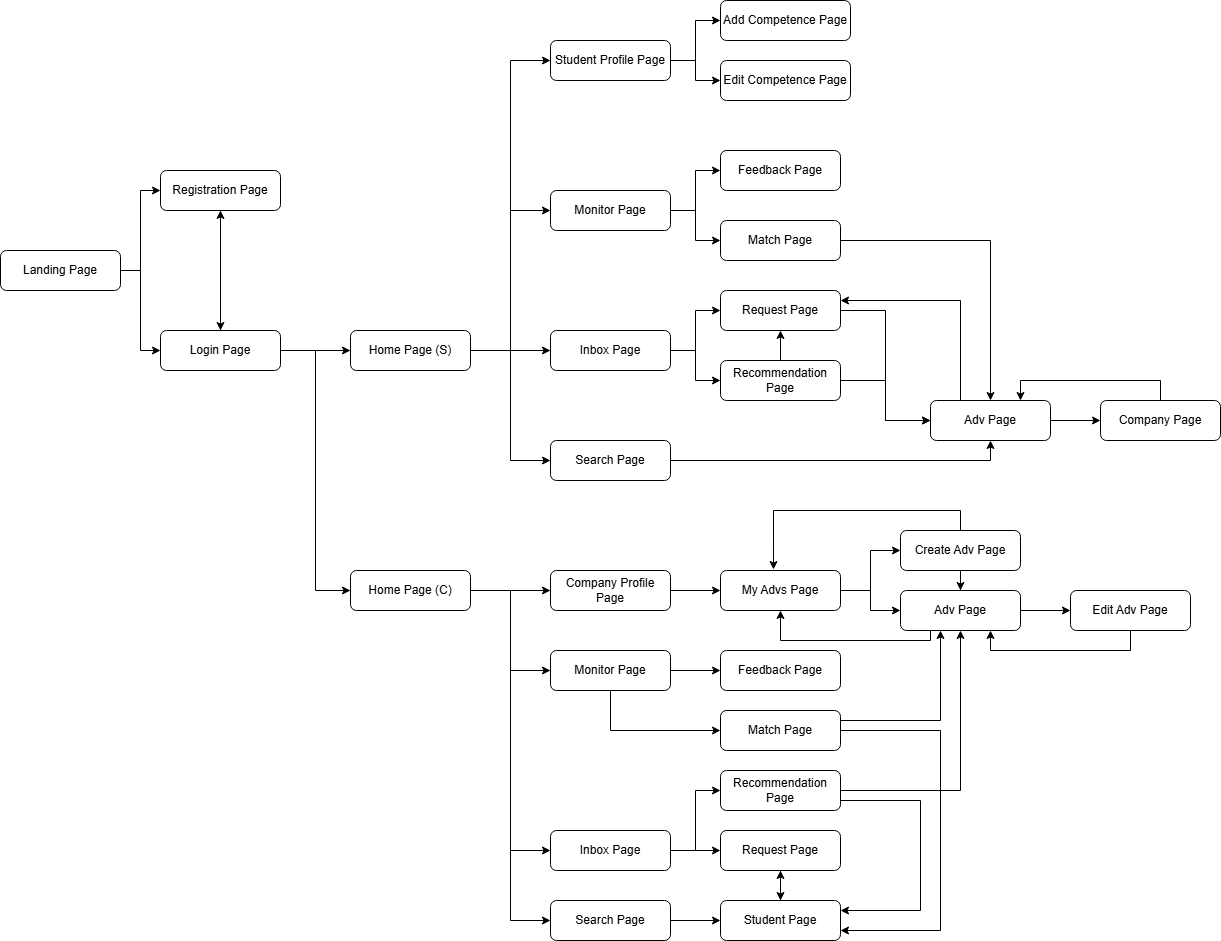
\includegraphics[width=15cm]{images/ui/DD-UI-Overview.drawio.png}
    \caption{User Interface Overview}
\end{figure}
This diagram shows how users can navigate the platform. Upon entering the website's URL, they are directed to the \textbf{Landing Page}, where they can choose between Registration and Login. Both pages allow users to switch to the other if needed. After logging in, users are redirected to their personalised \textbf{Home Page}, which varies depending on their role (S - Student, C - Company). A navigation bar is present on all pages, enabling users to move across the most relevant sections, i.e. \textbf{Profile Page}, \textbf{Monitor Page}, \textbf{Inbox Page}, and \textbf{Search Page}. The arrows in the diagram represent links between pages, but not all links are shown to maintain diagram clarity. Additionally, back buttons are available on each page to facilitate navigation.
When a student visits an \textbf{ADV Page}, they can send a request regarding that ADV (as shown by the arrow linking the Adv Page to the Request Page). Similarly, companies can perform the same action when viewing a student’s profile page.
Lastly, as discussed in the RASD document, users can provide feedback via the \textbf{Monitor Page}.
\section{Mock-up pages}
\subsection{Login Page}
\begin{figure}[H]
    \centering
    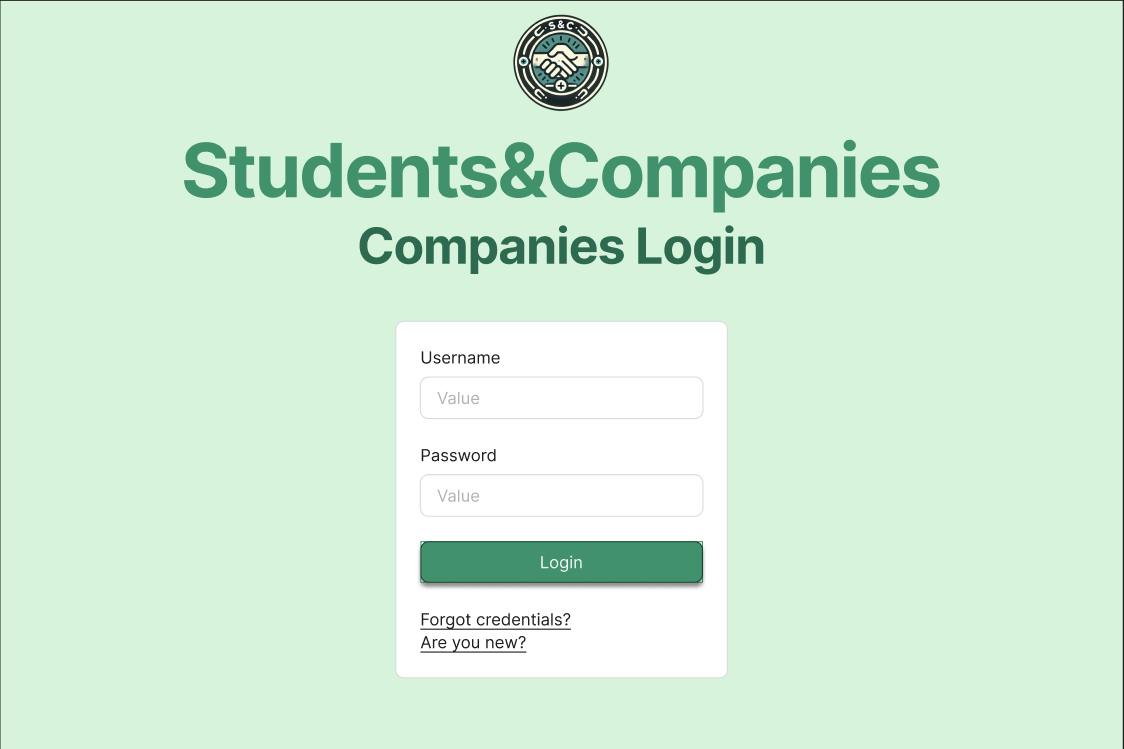
\includegraphics[width=15cm]{images/ui/login.jpg}
    \caption{UI: Login Page}
\end{figure}
This is the Login Page for companies. As precedent discussed, the company's representative can insert the username and the password given at the moment of registration. If they do not remember the password or the username, they can click on the "Forgot credentials?" link, they will have to insert their company email and they will be able to reset the credentials. If the company is not registered, the representative can click on the "Are you new?" link to be redirected to the Sign up Page.

The student's login page is not shown because similar.

\subsection{Sign Up Page}
\begin{figure}[H]
    \centering
    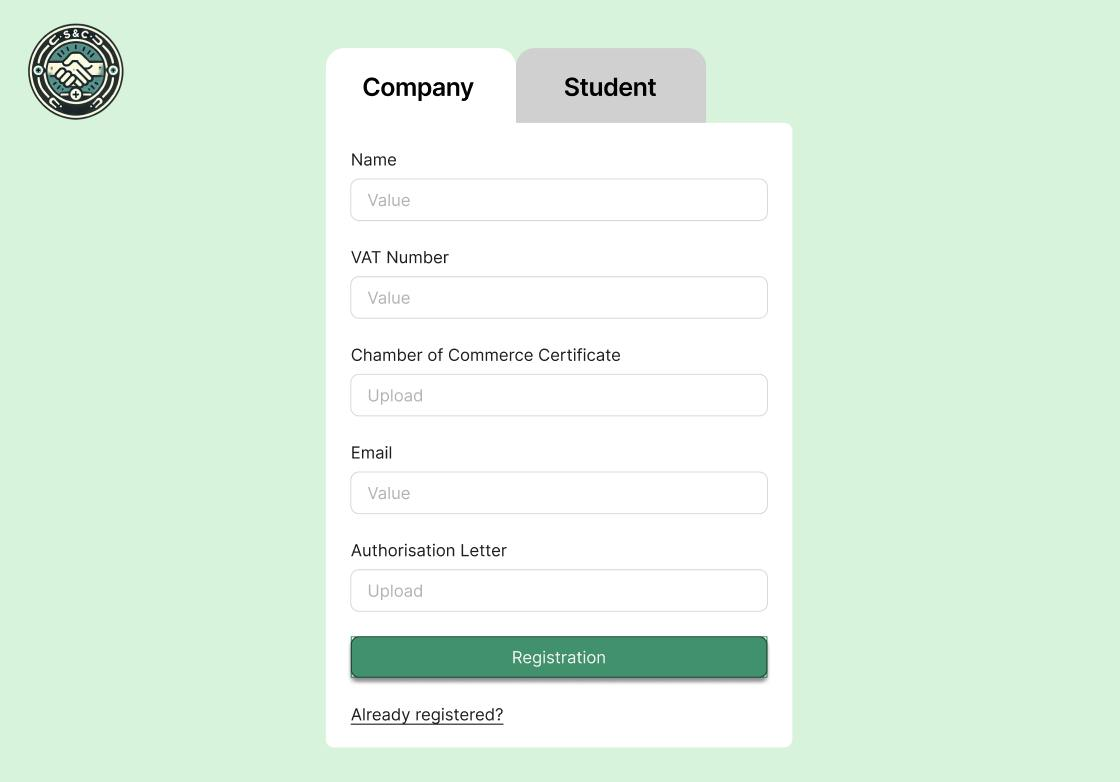
\includegraphics[width=15cm]{images/ui/signup.jpg}
    \caption{UI: Sign up Page}
\end{figure}
This is the form shown to companies that want to register to the platform. If someone is already registered, they can click on the "Already registered?" link and will be redirected to the Login Page. Students can click on the "Student" section to compile their form. This is not shown because is similar.

\subsection{Home Page}
\begin{figure}[H]
    \centering
    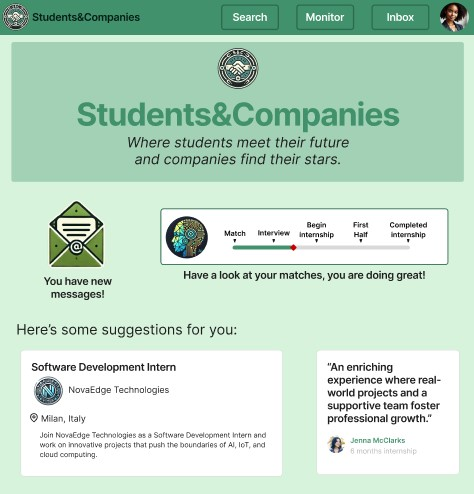
\includegraphics[width=15cm]{images/ui/homepage.jpg}
    \caption{UI: Home Page}
\end{figure}
The \textbf{navigation bar} contains the logo and the name of the platform, they are clickable and directs to the Home Page. The other buttons direct to the correspondent pages, and the profile picture directs to the profile.
The home page is personalised: in this case there is the envelope image that directs the user to the Inbox Page, and the monitor bar that redirects to the Monitor Page. The suggestions are linked to the Company Profile and to the ADV.

\subsection{Student Profile Page}
\begin{figure}[H]
    \centering
    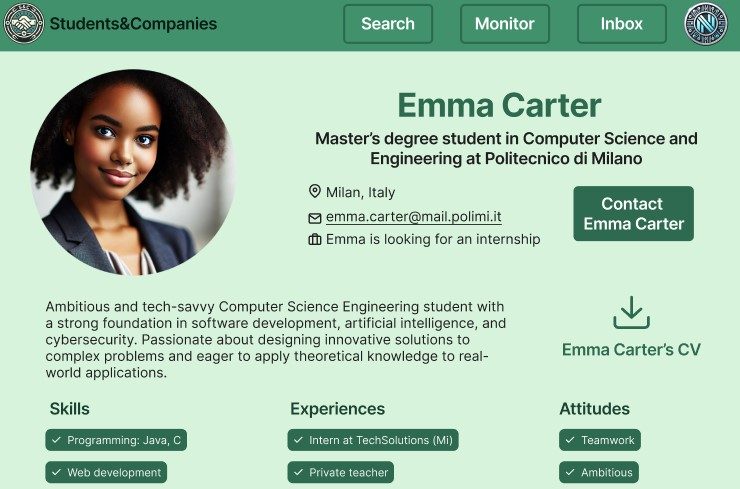
\includegraphics[width=15cm]{images/ui/studentprofile.jpg}
    \caption{UI: Student Profile Page}
\end{figure}
This is a student's Profile Page seen by a company. By clicking on the download icon or on the "Emma Carter's CV" link, a user can download the student's CV. By clicking on one of the shown competence, a pop-up window opens and shows the description inserted by the student. If a company is interested, they can click on the "Contact Emma Carter" button to send an Internship Request to the student. By scrolling the page all the competences are show, as well as relevant comments left by the companies.
\begin{figure}[H]
    \centering
    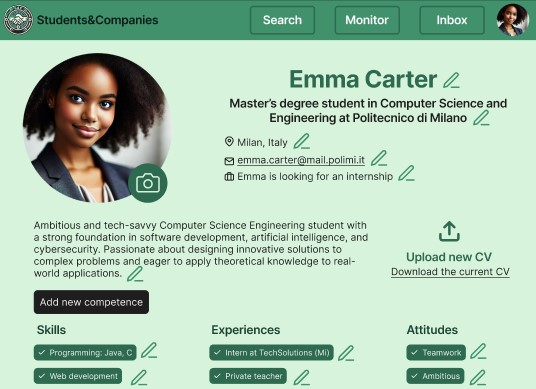
\includegraphics[width=15cm]{images/ui/studentprofilepersonal.jpg}
    \caption{UI: Student Personal Profile Page}
\end{figure}
This image shows how the student sees their own personal page. They can modify all the information by clicking on the pen icon, they can upload a new profile image by clicking on the camera icon, they can upload a new CV by clicking on the upload icon but also they can download the current one, and they can add a new competence by clicking on the button.

\subsection{Company Profile Page}
\begin{figure}[H]
    \centering
    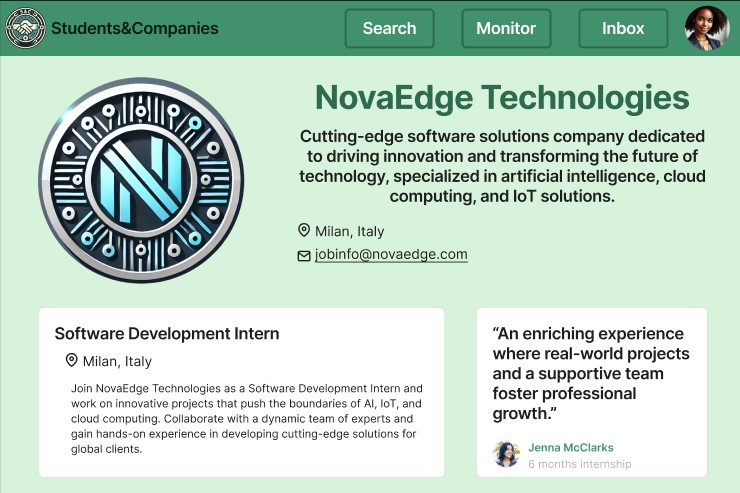
\includegraphics[width=15cm]{images/ui/companyprofile.jpg}
    \caption{UI: Company Profile Page}
\end{figure}
This is a company's profile seen by students. All the company's active ADVs are shown in the boxes on the left, they are clickable and bring the user to the ADV page. On the right, relevant comments by students are shown.

\subsection{Company's ADVs Page}
\begin{figure}[H]
    \centering
    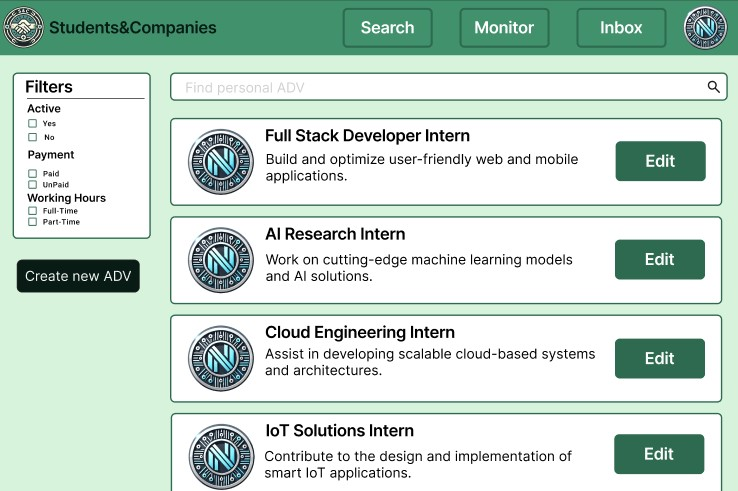
\includegraphics[width=15cm]{images/ui/advspage.jpg}
    \caption{UI: Company's ADVs Page}
\end{figure}
When a Company is logged in, the representative can reach the ADVs Page from the personal profile. A new ADV can be created by clicking on the button, and the other ones can be modified by clicking on the corresponding "Edit" button. ADVs can be found via the search bar and/or applying filters. The Interview Form can be created by clicking on the "Edit" button.

\subsection{Company's ADV Page}
\begin{figure}[H]
    \centering
    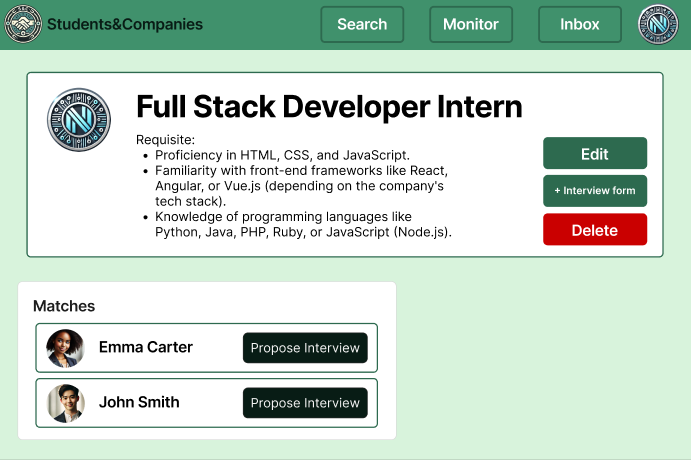
\includegraphics[width=15cm]{images/ui/advpage(1).png}
    \caption{UI: Company's ADV Page}
\end{figure}
When a Company is logged in, the representative can visualize ADV Page from the personal profile. The ADV can be edited by clicking on the "Edit" button, the representative can add a form to help the evaluation of the candidates during the interview by clicking on "+ Interview Form", or can delete the advertisement by clinking on "Delete" button. From this page the representative can also see all the students that has done a match with this Adv and setting up an interview with them pressing on "Propose Interview" button near the candidate name.


\subsection{ADV Page}
\begin{figure}[H]
    \centering
    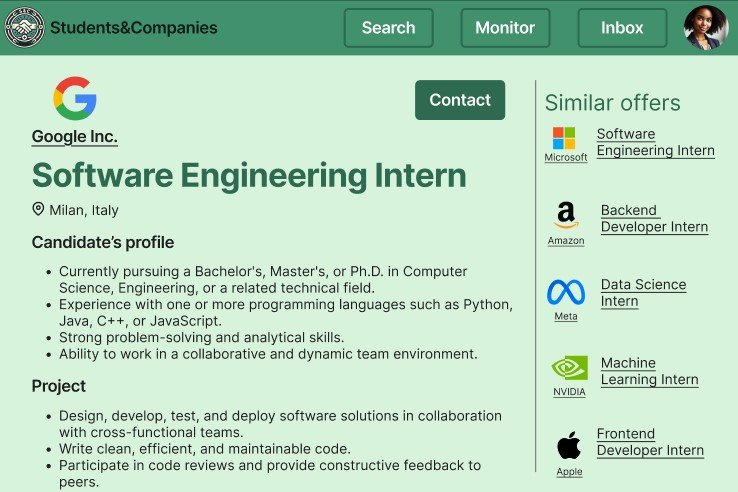
\includegraphics[width=15cm]{images/ui/advpage.jpg}
    \caption{UI: ADV Page}
\end{figure}
This is the ADV Page seen by students. It contains all the information about the Internship position (all viewable by scrolling the page). By clicking on the company's logo or the name, the student is redirected to the company's profile. A student can contact the company regarding this ADV by clicking on the "Contact" button. On the left links to similar offers are shown.

\subsection{Search Page}
\begin{figure}[H]
    \centering
    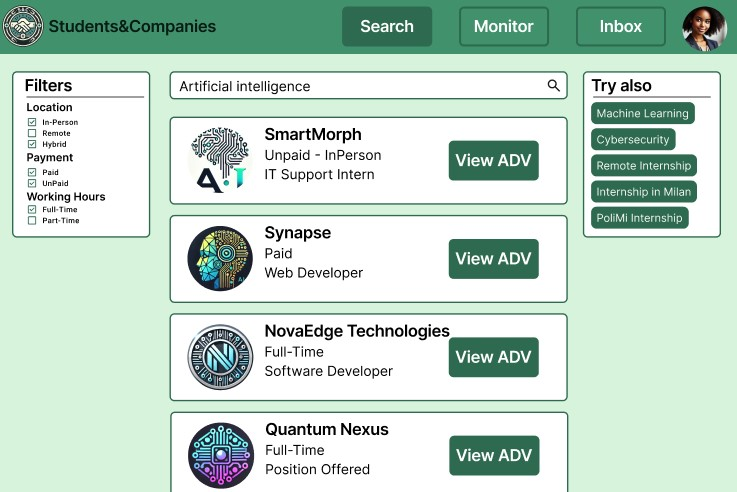
\includegraphics[width=15cm]{images/ui/search.jpg}
    \caption{UI: Search Page}
\end{figure}
The Search Page contains a search bar where the user (in this case a student) can insert key words. The user can also use the filters on the left or try the suggested key words on the right. When clicking on the "View ADV" button the student is redirected to the ADV page, while by clicking on the company's name they are redirected to the company's profile.

\subsection{Monitor Page}
\begin{figure}[H]
    \centering
    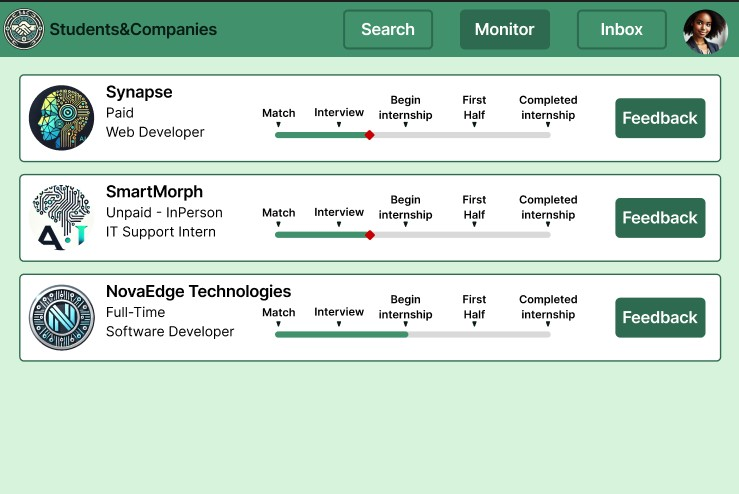
\includegraphics[width=15cm]{images/ui/monitor.jpg}
    \caption{UI: Monitor Page}
\end{figure}
The Monitor Page contains the match done, in this case it contains the ADV with which the student matched. For each ADV the student can see the progress and click on the "Feedback" button to leave one.
The companies Monitor Page first has the list of the ADVs, when clicking on one of them the company is redirected to the monitor page of that ADV so they will see a list of student that have match with that adv, just as the image above.

\subsection{Inbox Page}
\begin{figure}[H]
    \centering
    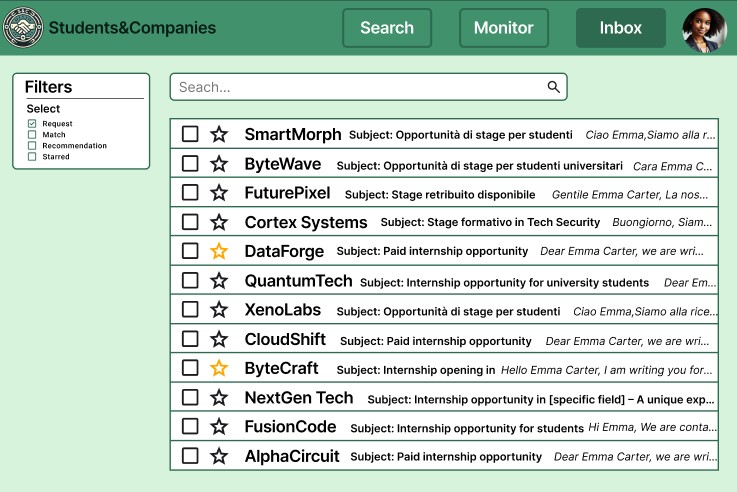
\includegraphics[width=15cm]{images/ui/inbox.jpg}
    \caption{UI: Inbox Page}
\end{figure}
This is the Inbox Page, it works as a standard mail box. 